\documentclass[10pt,a4paper,german]{article}
\usepackage[utf8]{inputenc}
\usepackage{amsmath}
\usepackage{amsfonts}
\usepackage{amssymb}
\usepackage{graphicx,caption}
\usepackage{float}

\setlength\parindent{0pt}

\begin{document}
\section{Bildverarbeitung}
\subsection{JPEG Verarbeitung}
Die Aufnahmen der Kamera werden von der Software standardmäßig als JPEG Dateien abgespeichert.
Dies ist für eine weitere quantitative Auswertung problematisch, da die gemessenen Temperaturen in RGB-Werte umgewandelt werden.
Zusätzlich ist die Erstellung von JPEG Dateien mit dem Verlust von Bildinformation gekoppelt. 
Dementsprechend ist es für eine quantitative Auswertung notwendig die ursprünglichen Temperaturinformationen für jeden Pixel möglichst genau wiederherzustellen.
Dies wird in zwei Schritten bewerkstelligt:
Einerseits der Zuordnung von Farb- und Temperaturwerten mittels des im Bild inkludierten Farbbalkens, andererseits der Umwandlung aller Pixel in Temperaturen.

\subsubsection{Farb-Temperatur Zuordnung}

\begin{center}
    $<$ Bild - Beispielbild $>$
\end{center}

Jedes Bild verfügt über eine Farbskala, welche zum visuellen Abschätzen der Temperaturen innerhalb des Bildes dient.
Bei der Wahl des Aufnahmemodus ist es wichtig eine lineare Farbskala zu verwenden, da es andernfalls nicht möglich ist ein genaue Temperaturzuordnung zu finden.
Der Maximal- und Minimalwert der Skala ist in der App jeweils mit der entsprechenden Temperatur gekennzeichnet.
Mit Hilfe dieser Informationen lässt sich eine Zuordnung von Farbwert und Temperatur erzeugen.
Für jeden Pixel $i$ des Farbbalkens kann die korrespondierende Temperatur $T_{scale,i}$ mittels folgender Formel berechnet werden:

\begin{equation}
    T_{scale,i} = \frac{i}{n} \left(T_{max} - T_{min}\right) + T_{min}
\end{equation}

wobei $n$ die Anzahl der Pixel des Farbbalkens repräsentiert.
Die beiden angegebenen Randtemperaturen $T_{min}$ und $T_{max}$ werden jeweils ganzzahlig angegebenen.
Dies lässt die Frage offen, ob diese zur Präsentation auf- oder abgerundet wurden.
Die Standardunsicherheit der Randtemperaturen $u_{round}$ kann quantifiziert werden durch:

\begin{equation}
    u_{round} = \frac{1}{2\sqrt{3}}
\end{equation}

Folglich ergibt sich ein möglicher Fehler für die berechneten Temperaturen, welcher sich über die Fehlerfortpflanzung berechnen lässt:

\begin{equation}
    u_{scale,i} = \sqrt{\left(\frac{i}{n} u_{round} \right)^2 + \left(\left(1 - \frac{i}{n}\right) u_{round}\right)^2}
\end{equation}

Hier beschreibt $u_{scale,i}$ die Standardunsicherheit des berechneten Temperaturwerts der $i$-ten Balkenfarbe.

\subsubsection{Farbinterpolation}
Nun sind zwar die Temperaturen für alle Farben der Farbskala bekannt, jedoch können die Pixel des eigentlichen Bildes Farbwerte besitzen, die zwischen jenen der Skala liegen.
Mit Hilfe von Interpolation lassen sich auch diesen Farben Temperaturen zuordnen.
Im Allgemeinen ist die Interpolation von RGB Werten jedoch keine einfache Aufgabe. 
Der Farbverlauf der Skala stellt eine dreidimensionale Kurve im RGB-Raum dar, welche auf Grund des JPEG Formats über ungenaue Farbwerte verfügt.
Dies schließt die Anwendung vieler der üblicher Interpolationsmethoden aus.
Eine mögliche Variante ist der Einsatz von Nearest-Neighbor Interpolation, welche allerdings zu einem zusätzlichen Interpolationsfehler führt.
\\
\\
Alternativ kann durch die Verwendung einer schwarz-weißen Farbskala das Problem der Farbinterpolation im gesamten Umgangen werden.
In diesem Fall liegen alle Farbwerte auf einer eindeutig definierten Linie, wodurch lineare Interpolation ein präzises Ergebnis liefert.

\begin{figure}[H]
    \centering
    \captionsetup{width=8cm}
    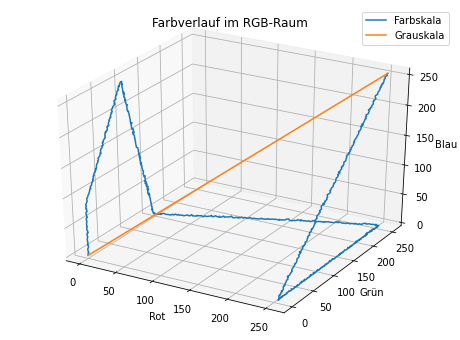
\includegraphics[width=10cm]{img/farb_vs_grau.png}
    \caption{Vergleich der Kurve einer Farbskala und einer Grauskala im RGB-Raum.}
\end{figure}

\subsection{TIFF Verarbeitung}
Die Wahl der entsprechenden Einstellung in der Seek Thermal App ermöglicht es aufgenommene Bilder im TIFF Format abzuspeichern. 
Dieses Bildformat ist in der Lage mehrere Bilder in eine Datei zusammenzufassen.
Im Falle der Seek App befinden sich darunter auch die gemessenen unveränderten Temperaturwerte.
Dementsprechend entfällt die Notwendigkeit die Temperaturen von den Farbwerten der Pixel abzuleiten.
Der relative Fehler jedes Temperaturwertes ist in diesem Fall rein von der thermischen Messgenauigkeit der Kamera bestimmt.
Eine Internetrecherche für das Modell "Seek Compact XR" ergibt eine Temperaturtoleranz $tol_{th} = 0.07 ^{\circ}C$.
Die entsprechende Standardunsicherheit berechnet sich mit:

\begin{equation}
    u_{th} = \frac{tol_{th}}{2\sqrt{3}}
\end{equation}

\section{Emissionsgradbestimmung}
Im Falle eines schwarzen Körpers ist die von der Kamera erfasste Strahlungsleistung definiert durch:

\begin{equation}
    P(T) = \sigma f T^4
\end{equation}

Die reale erfasste Strahlungsleistung kann vereinfacht mittels des Emissionsgrades ausgedrückt werden. 
Der Anteil der reflektierten Strahlung kann während der Versuche als konstant angenommen werden.
Dementsprechend kann aus der Differenz zwischen der gemessenen Temperatur $T_\textit{sens}$ und tatsächlichen Temperatur $T_\textit{obj}$ aus zwei Versuchen der Emissionsgrad $\epsilon$ berechnet werden.

\begin{equation}
    P(T_\textit{sens}) = \epsilon \cdot P(T_\textit{obj}) + (1 - \epsilon) \cdot P(T_\textit{env})
\end{equation}

\begin{equation}
   T_\textit{sens}^4 = \epsilon \cdot T_\textit{obj}^4 + (1 - \epsilon) \cdot T_\textit{env}^4
\end{equation}

\begin{equation}
    T_\textit{sens}^4 - \epsilon \cdot T_\textit{obj}^4 = (1 - \epsilon) \cdot T_\textit{env}^4 = C = \textit{const.}
\end{equation}

\begin{equation}
    T_\textit{sens,1}^4 - \epsilon \cdot T_\textit{obj,1}^4 = T_\textit{sens,2}^4 - \epsilon \cdot T_\textit{obj,2}^4 
\end{equation}

\begin{equation}
    \epsilon = \frac{T_\textit{sens,1}^4 - T_\textit{sens,2}^4}{T_\textit{obj,1}^4 - T_\textit{obj,2}^4}
\end{equation}

Da der Emissionsgrad der Referenzstelle ($\epsilon_\textit{obj}$) bekannt ist, kann der Emissionsgrad der Kamera ($\epsilon_\textit{sens}$) berechnet werden.
Weiters kann für das gesamte Bild der Emissionsgrad jedes einzelnen Pixel bestimmt werden.
Diese Werte beziehen sich auf die tatsächliche Temperatur des Körpers $T_\textit{obj}$ und sind nur für diesen gültig.

\begin{equation}
    \epsilon_\textit{sens} = \frac{\epsilon}{\epsilon_\textit{obj}}
\end{equation}

\begin{equation}
    \epsilon_\textit{pixel} = \frac{T_\textit{pixel}^4 - C}{\epsilon_\textit{sens} \cdot T_\textit{obj}^4}
\end{equation}

\begin{figure}[H]
    \centering
    \captionsetup{width=12cm}
    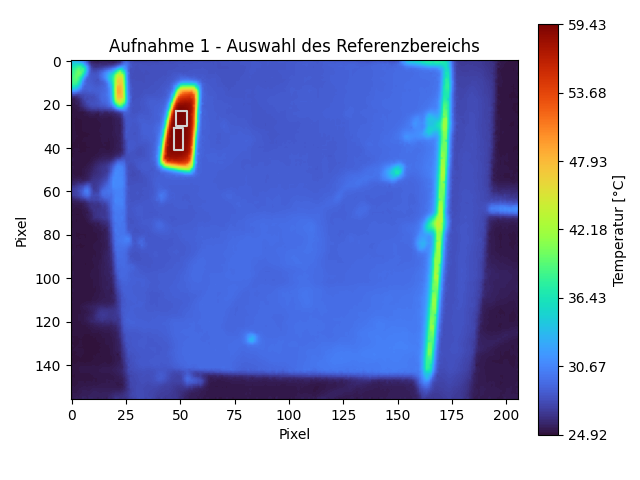
\includegraphics[width=6cm]{img/ref_sel_1.png}
    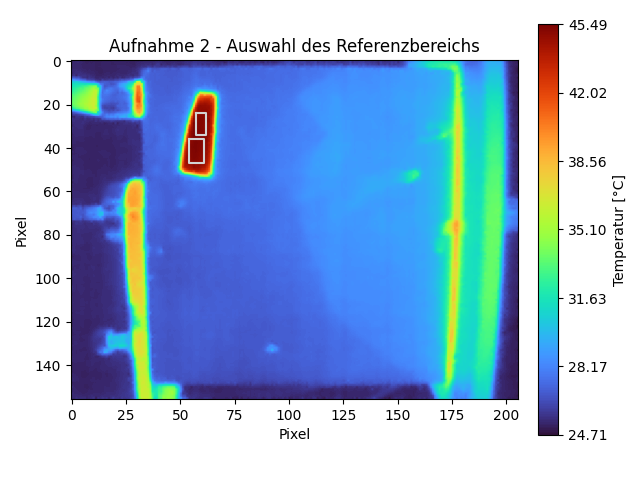
\includegraphics[width=6cm]{img/ref_sel_2.png}
    \caption{Auswahl eines Referenzbereiches (graue Rechtecke) mit bekanntem Emissionsgrad für beide Bilder.}
\end{figure}

\begin{figure}[H]
    \centering
    \captionsetup{width=12cm}
    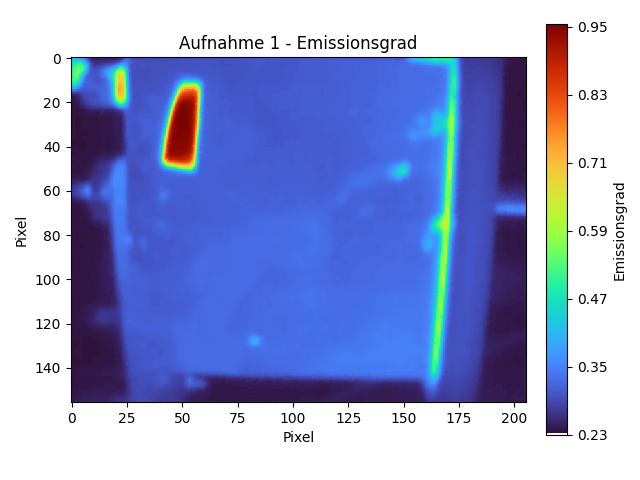
\includegraphics[width=6cm]{img/eps_1.png}
    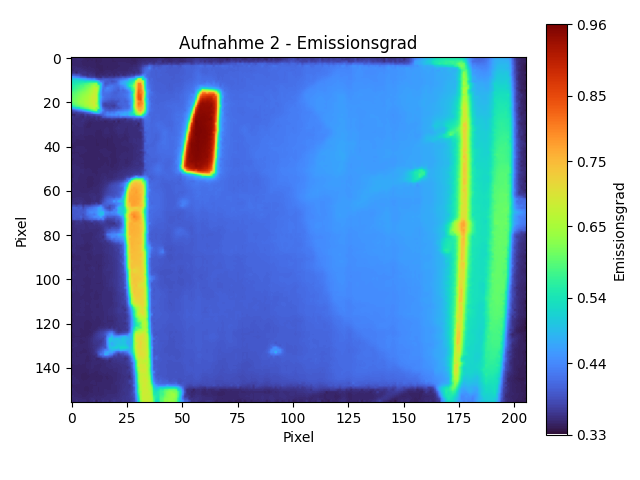
\includegraphics[width=6cm]{img/eps_2.png}
    \caption{Der berechnete Emissionsgrad für jeden Pixel der beiden Bilder.}
\end{figure}

Zur Kontrolle des berechneten Emissionsgrades kann rückwirkend die Temperatur des Körpers berechnet werden.
Im Idealfall zeigt der gesamte Körper die gleiche Temperatur.

\begin{equation}
    T_\textit{pixel,corr} = \sqrt[4]{\frac{T_\textit{pixel}^4 - C}{\epsilon_\textit{pixel} \cdot \epsilon_\textit{sens}}}
\end{equation}

\begin{center}
    $<$BILD - Temperatur korrigiert$>$
\end{center}


\end{document}